\documentclass[tikz,border=8pt]{standalone}
% Shared look for every TikZ diagram. Load with % Shared look for every TikZ diagram. Load with % Shared look for every TikZ diagram. Load with \input{../../tools/tikz-style.tex}
\usepackage[T1]{fontenc}
\usepackage{lmodern}
\renewcommand{\sfdefault}{lmr}  % diagrams use the same serif as the text
\usetikzlibrary{arrows.meta, positioning, shapes.geometric, calc, fit, backgrounds}
\definecolor{cblue}{HTML}{4C78A8}
\definecolor{corange}{HTML}{F58518}
\definecolor{cgreen}{HTML}{54A24B}
\definecolor{cred}{HTML}{E45756}
\definecolor{cpurple}{HTML}{B279A2}
\definecolor{cgrey}{HTML}{6B6B6B}
\tikzset{
  every picture/.style={font=\sffamily, line width=1.2pt},
  box/.style={draw=#1, fill=#1!12, rounded corners=4pt, align=center, inner sep=7pt, minimum height=1.1cm},
  box/.default=cgrey,
  arrow/.style={-{Stealth[length=3mm]}, draw=cgrey, line width=1.4pt},
  title/.style={font=\sffamily\bfseries\Large},
  note/.style={font=\sffamily\small, text=cgrey, align=center},
}
\AtBeginDocument{\hyphenpenalty=10000 \exhyphenpenalty=10000}

\usepackage[T1]{fontenc}
\usepackage{lmodern}
\renewcommand{\sfdefault}{lmr}  % diagrams use the same serif as the text
\usetikzlibrary{arrows.meta, positioning, shapes.geometric, calc, fit, backgrounds}
\definecolor{cblue}{HTML}{4C78A8}
\definecolor{corange}{HTML}{F58518}
\definecolor{cgreen}{HTML}{54A24B}
\definecolor{cred}{HTML}{E45756}
\definecolor{cpurple}{HTML}{B279A2}
\definecolor{cgrey}{HTML}{6B6B6B}
\tikzset{
  every picture/.style={font=\sffamily, line width=1.2pt},
  box/.style={draw=#1, fill=#1!12, rounded corners=4pt, align=center, inner sep=7pt, minimum height=1.1cm},
  box/.default=cgrey,
  arrow/.style={-{Stealth[length=3mm]}, draw=cgrey, line width=1.4pt},
  title/.style={font=\sffamily\bfseries\Large},
  note/.style={font=\sffamily\small, text=cgrey, align=center},
}
\AtBeginDocument{\hyphenpenalty=10000 \exhyphenpenalty=10000}

\usepackage[T1]{fontenc}
\usepackage{lmodern}
\renewcommand{\sfdefault}{lmr}  % diagrams use the same serif as the text
\usetikzlibrary{arrows.meta, positioning, shapes.geometric, calc, fit, backgrounds}
\definecolor{cblue}{HTML}{4C78A8}
\definecolor{corange}{HTML}{F58518}
\definecolor{cgreen}{HTML}{54A24B}
\definecolor{cred}{HTML}{E45756}
\definecolor{cpurple}{HTML}{B279A2}
\definecolor{cgrey}{HTML}{6B6B6B}
\tikzset{
  every picture/.style={font=\sffamily, line width=1.2pt},
  box/.style={draw=#1, fill=#1!12, rounded corners=4pt, align=center, inner sep=7pt, minimum height=1.1cm},
  box/.default=cgrey,
  arrow/.style={-{Stealth[length=3mm]}, draw=cgrey, line width=1.4pt},
  title/.style={font=\sffamily\bfseries\Large},
  note/.style={font=\sffamily\small, text=cgrey, align=center},
}
\AtBeginDocument{\hyphenpenalty=10000 \exhyphenpenalty=10000}

% Section 10: student 1 (true class yes, softmax output 0.2, 0.3, 0.5). One-hot label: three products, two of them 0.
% Integer label 0: pick one probability. Same loss, 1.609.
\begin{document}
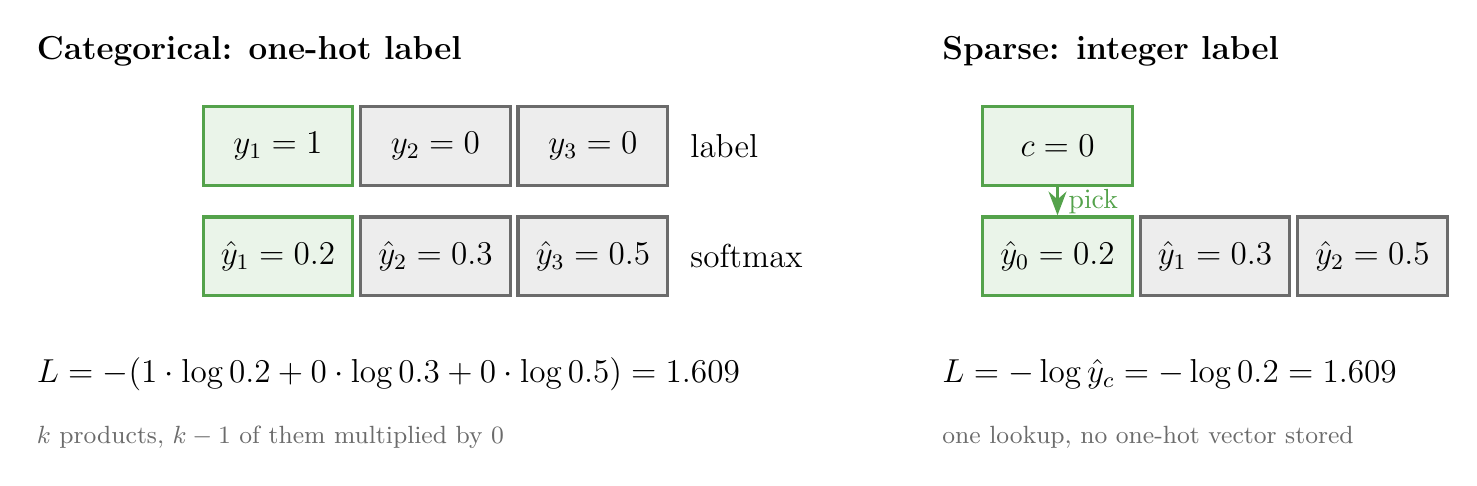
\begin{tikzpicture}[cell/.style={draw=#1, fill=#1!12, minimum width=1.9cm, minimum height=1cm, font=\large},
                    lab/.style={font=\large\bfseries}]
  % categorical
  \node[lab, anchor=west] at (-1.2, 2.2) {Categorical: one-hot label};
  \foreach \v/\c [count=\i] in {1/cgreen, 0/cgrey, 0/cgrey} \node[cell=\c] (y\i) at (2.0*\i, 1) {$y_\i = \v$};
  \foreach \v/\c [count=\i] in {0.2/cgreen, 0.3/cgrey, 0.5/cgrey} \node[cell=\c] (p\i) at (2.0*\i, -0.4) {$\hat y_\i = \v$};
  \node[font=\large, anchor=west] at (7.1, 1) {label};
  \node[font=\large, anchor=west] at (7.1, -0.4) {softmax};
  \node[font=\large, align=left, anchor=west] at (-1.2, -1.9)
    {$L = -(1 \cdot \log 0.2 + 0 \cdot \log 0.3 + 0 \cdot \log 0.5) = 1.609$};
  \node[note, anchor=west] at (-1.2, -2.7) {$k$ products, $k - 1$ of them multiplied by 0};
  % sparse
  \begin{scope}[xshift=11.5cm]
    \node[lab, anchor=west] at (-1.2, 2.2) {Sparse: integer label};
    \node[cell=cgreen] (c) at (0.4, 1) {$c = 0$};
    \foreach \v/\c [count=\i from 0] in {0.2/cgreen, 0.3/cgrey, 0.5/cgrey} \node[cell=\c] (q\i) at (2.0*\i+0.4, -0.4) {$\hat y_\i = \v$};
    \draw[arrow, draw=cgreen] (c) -- node[right, font=\normalsize, text=cgreen] {pick} (q0);
    \node[font=\large, align=left, anchor=west] at (-1.2, -1.9) {$L = -\log \hat y_c = -\log 0.2 = 1.609$};
    \node[note, anchor=west] at (-1.2, -2.7) {one lookup, no one-hot vector stored};
  \end{scope}
\end{tikzpicture}
\end{document}
